\subsubsection{Análisis de desempeño}
Algunas de las instancias del problema de Enrutamiento de Vehículos con Capacidad pueden brindar una solución muy distante de la óptima utilizando este algoritmo debido a las heurísticas que se utilizan. A continuación mencionaremos algunas:

\subsubsubsection{Camiones que ``van y vienen''}
La primera decisión del algoritmo es ordenar los vértices por demanda y luego cada \textit{bucket} por cercanía al depósito para finalmente obtener un \textit{bucket} de vértices satisfacibles por el stock de un camión. Consideremos este \textit{bucket} $B$ (que recordamos es una lista de vértices). Es posible que los $K$ elementos de $B$ más cercanos al depósito no estén cerca del último nodo $v$ visitado por el camión actual, sino por el contrario; estén en esquinas opuestas. Luego, al ordenar estos $K$ elementos por la distancia a $v$, los camiones recorrerán distancias muy largas con total de cumplir la heurística de satisfacer primero las demandas más altas. A continuación analizamos este caso gráficamente:

\begin{figure}[H]
	\centering
	\begin{minipage}{0.48\textwidth}
		\centering
		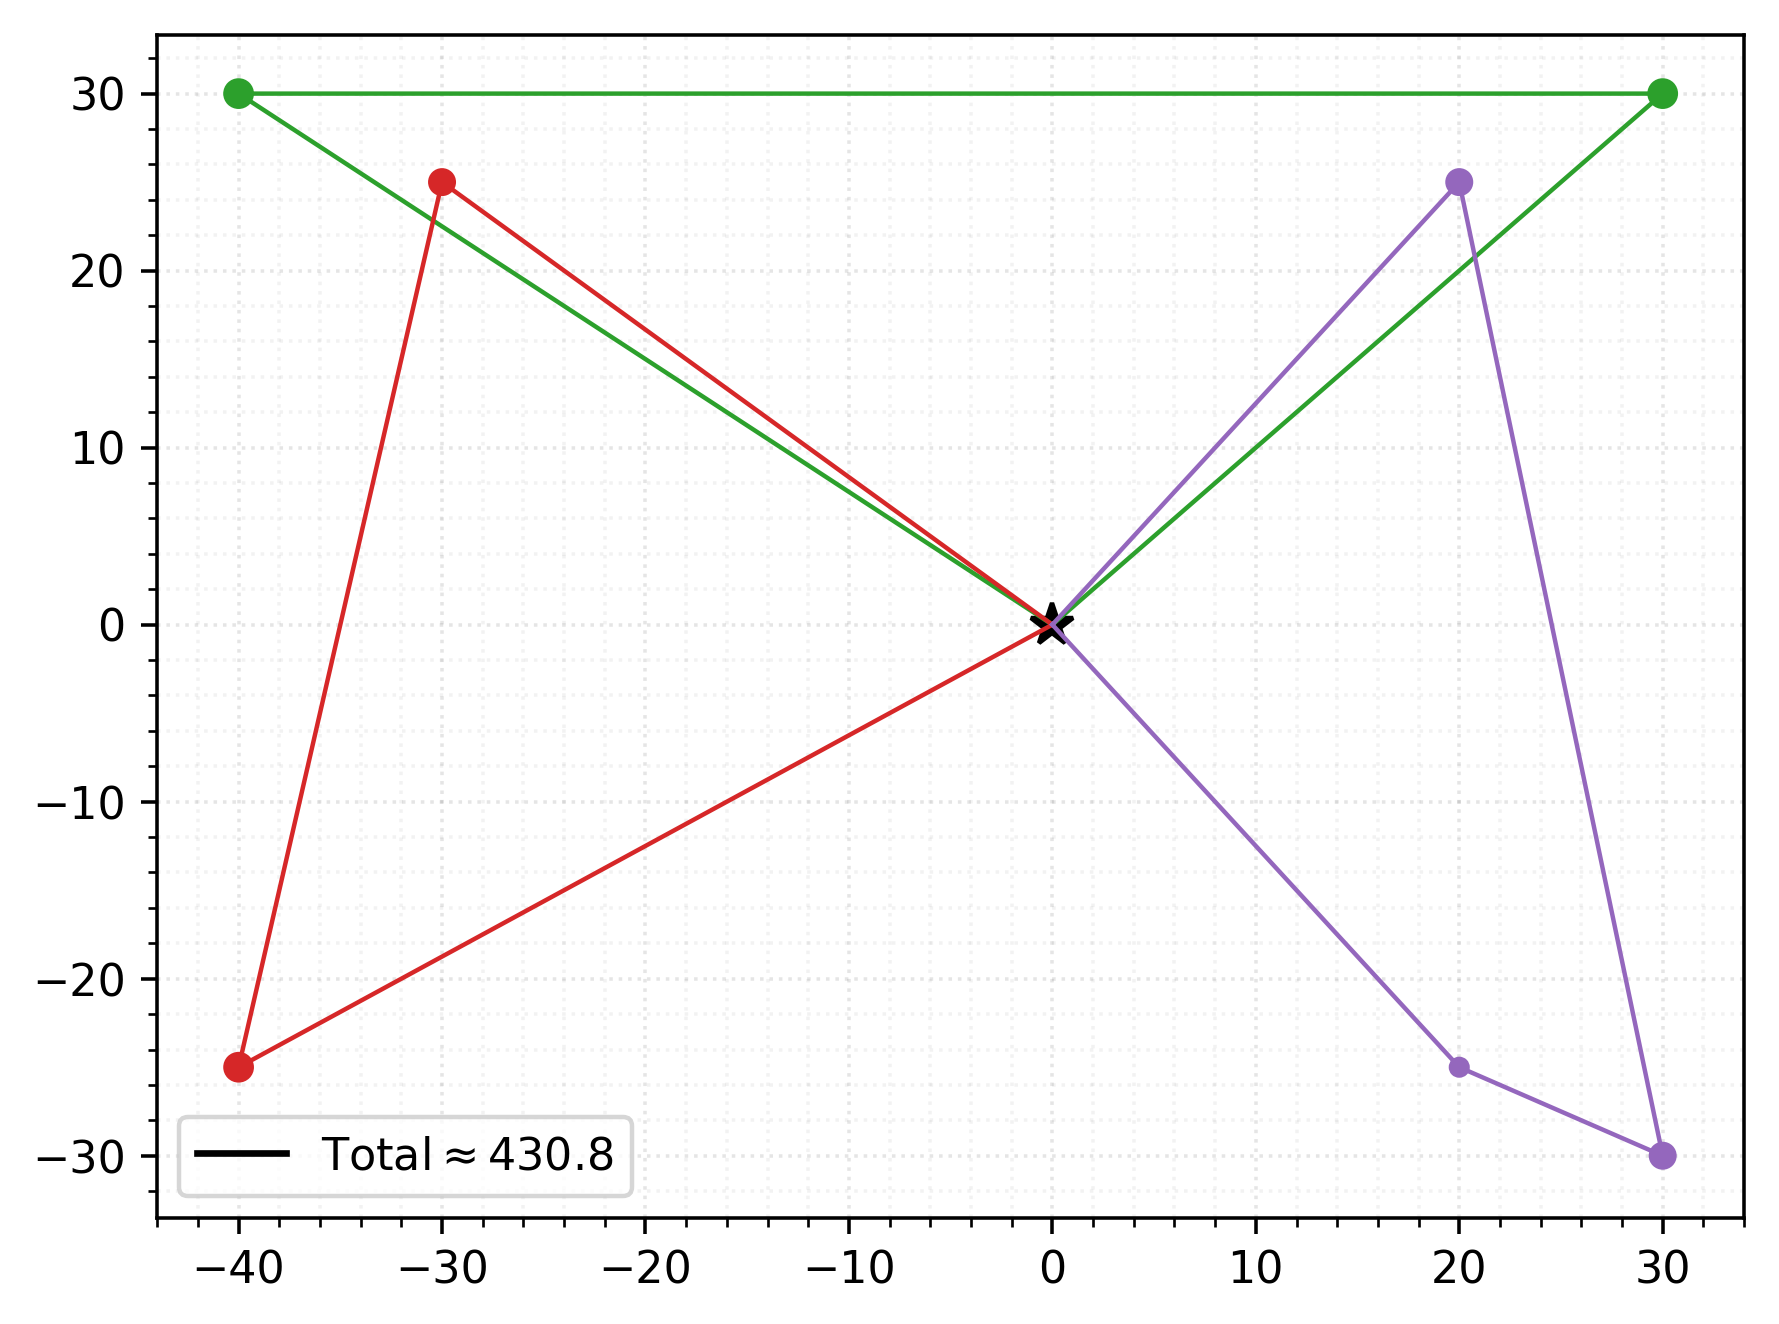
\includegraphics[width=1\textwidth]{greedy/gr-custom-n9-greedy-worst-case-K4}
		\caption{\footnotesize Solución no óptima mediante el algoritmo \textbf{goloso constructivo}. Capacidad 100.}
		\label{fig:sa-custom-n9-greedy-worst-case-K4}
	\end{minipage}%
	\hspace{0.03\textwidth}
	\begin{minipage}{0.48\textwidth}
		\centering
		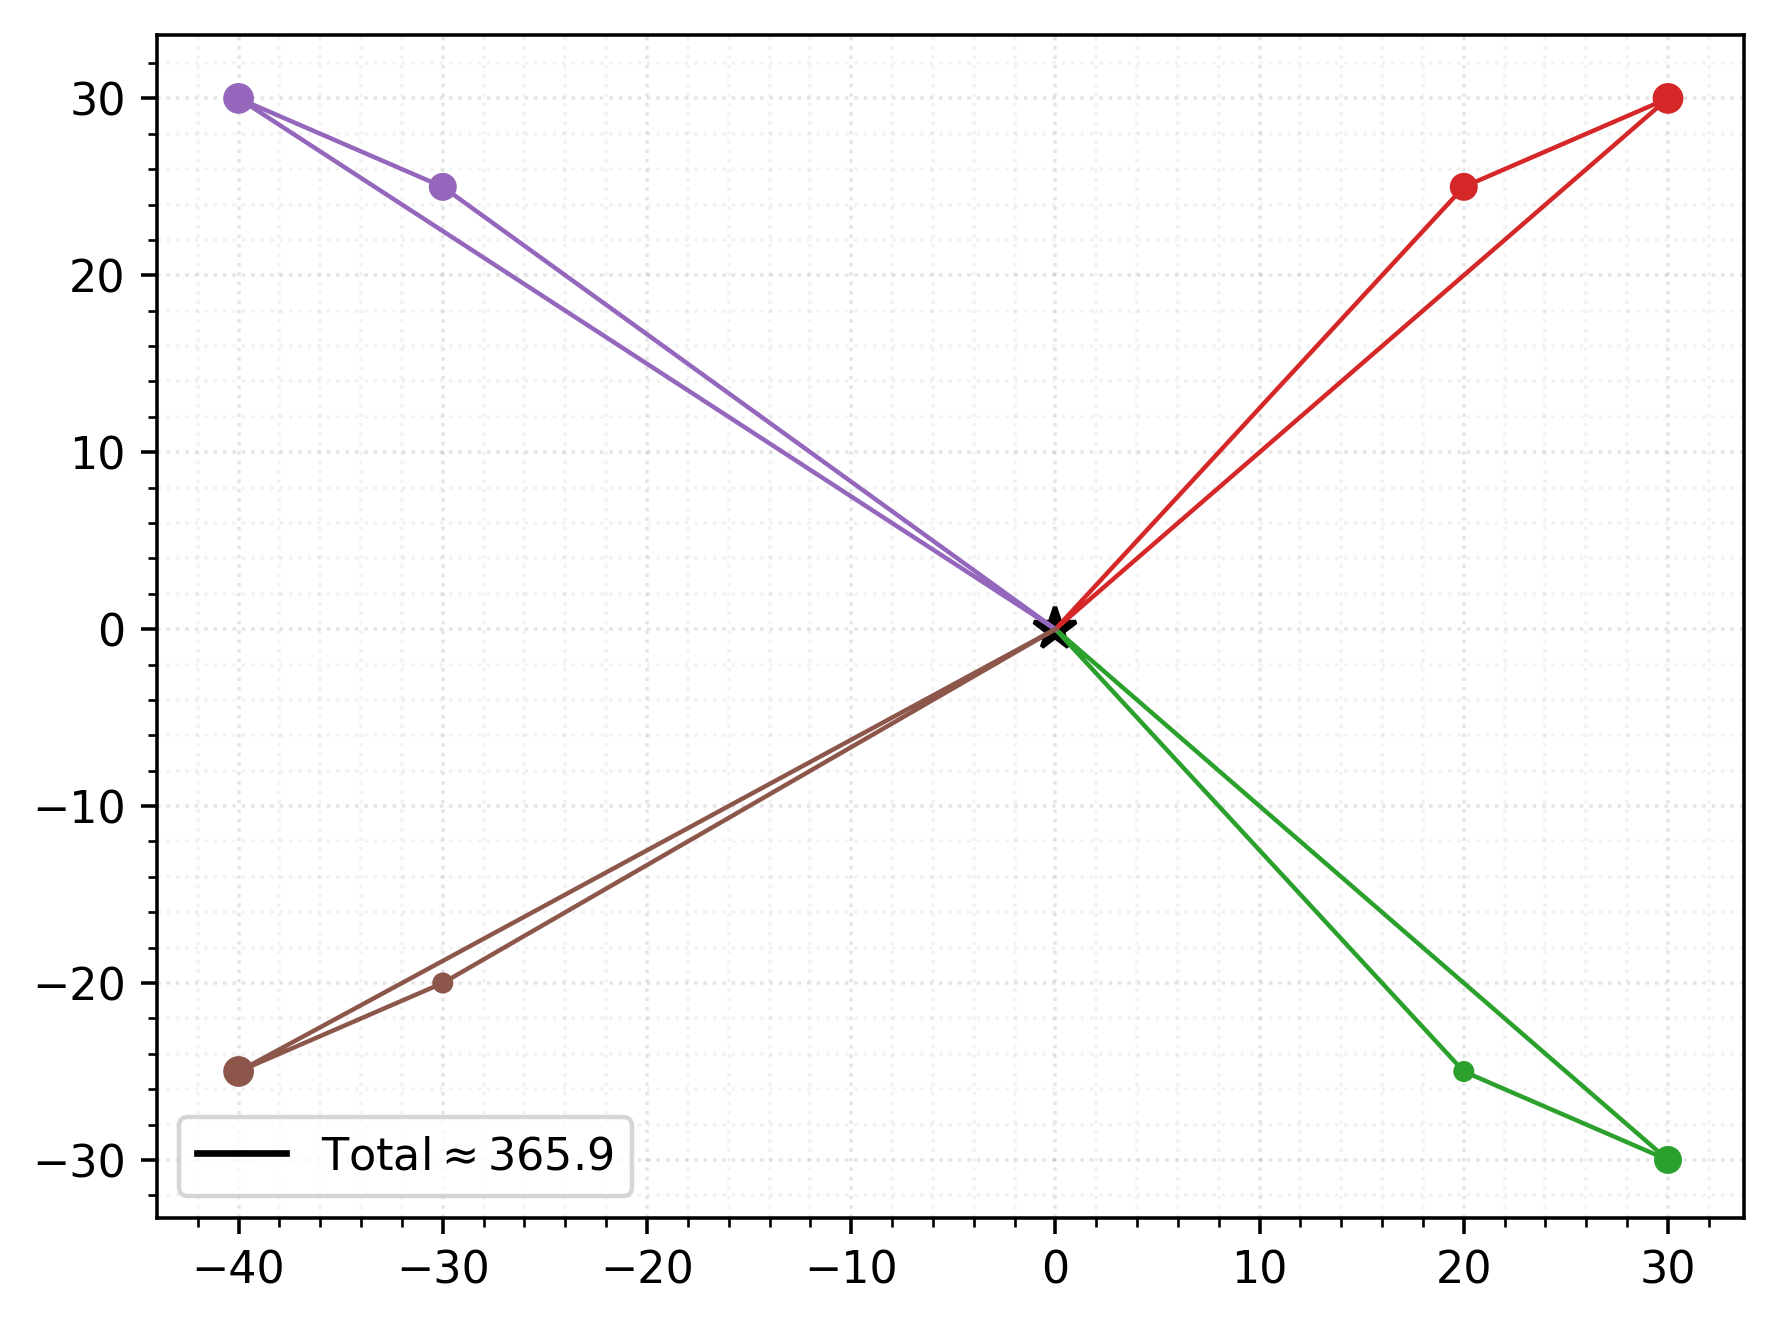
\includegraphics[width=1\textwidth]{greedy/sw-custom-n9-greedy-worst-case}
		\caption{\footnotesize Solución óptima mediante el algoritmo \textbf{Clusterize (sweep), route (nearest neighbours)}. Capacidad 100.}
		\label{fig:sw-custom-n9-greedy-worst-case-K4}
	\end{minipage}%
\end{figure}

En los gráficos, los nodos más gruesos representan demandas mayores. Como es posible de analizar, en la solución golosa constructiva, se decide realizar rutas conectando los vértices más demandantes posibles. Debido a esto se comete una planificación ineficiente. En cambio, el algoritmo \textbf{clusterize first, route second} que será abordado en el futuro, no tuvo problemas encontrando la solución óptima pues no posee heurísticas interesadas en las demandas de los clientes.

\subsubsubsection{Demandas equivalentes}
Otro caso inoportuno para el algoritmo podría presentarse en forma de demandas equivalentes, donde ordenar por demanda no ofrezca absolutamente ninguna ventaja pues todas son iguales. Además, los vértices se terminarían ordenando por cercanía al depósito donde pueden ocurrir problemas como el de ``van y vienen'' explicado en el punto anterior.

\begin{figure}[H]
	\centering
  \label{fig:sgr-custom-n32-equal-demands}
  \caption{\footnotesize Vértices con demandas equivalentes (todas valen $20$) y capacidad de camión $100$}
	\begin{minipage}{0.30\textwidth}
		\centering
		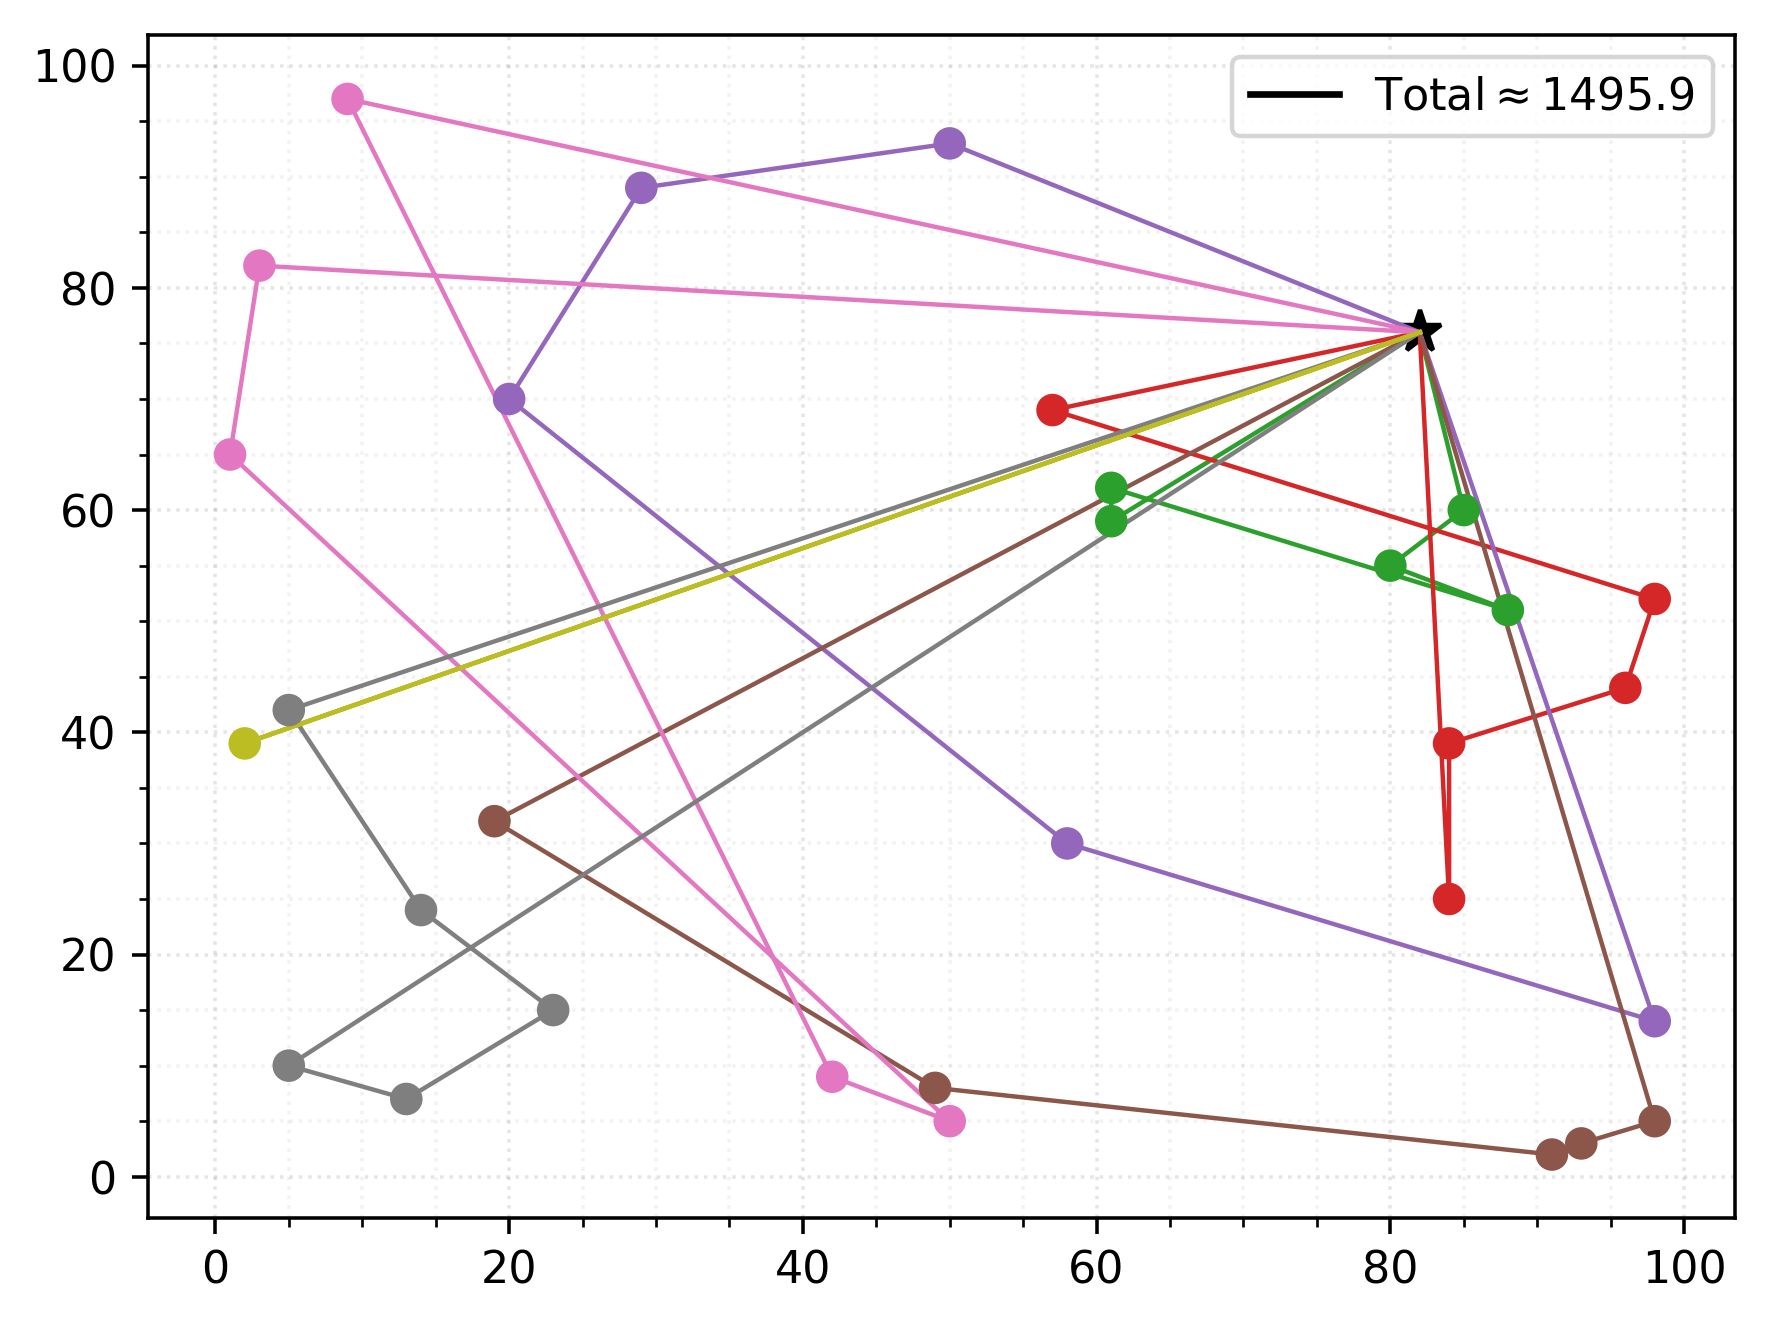
\includegraphics[width=1\textwidth]{greedy/gr-custom-n32-equal-demands-K1}
		\footnotesize \textbf{(a)} $K = 1$
	\end{minipage}%
  \hspace{0.03\textwidth}
	\begin{minipage}{0.30\textwidth}
		\centering
		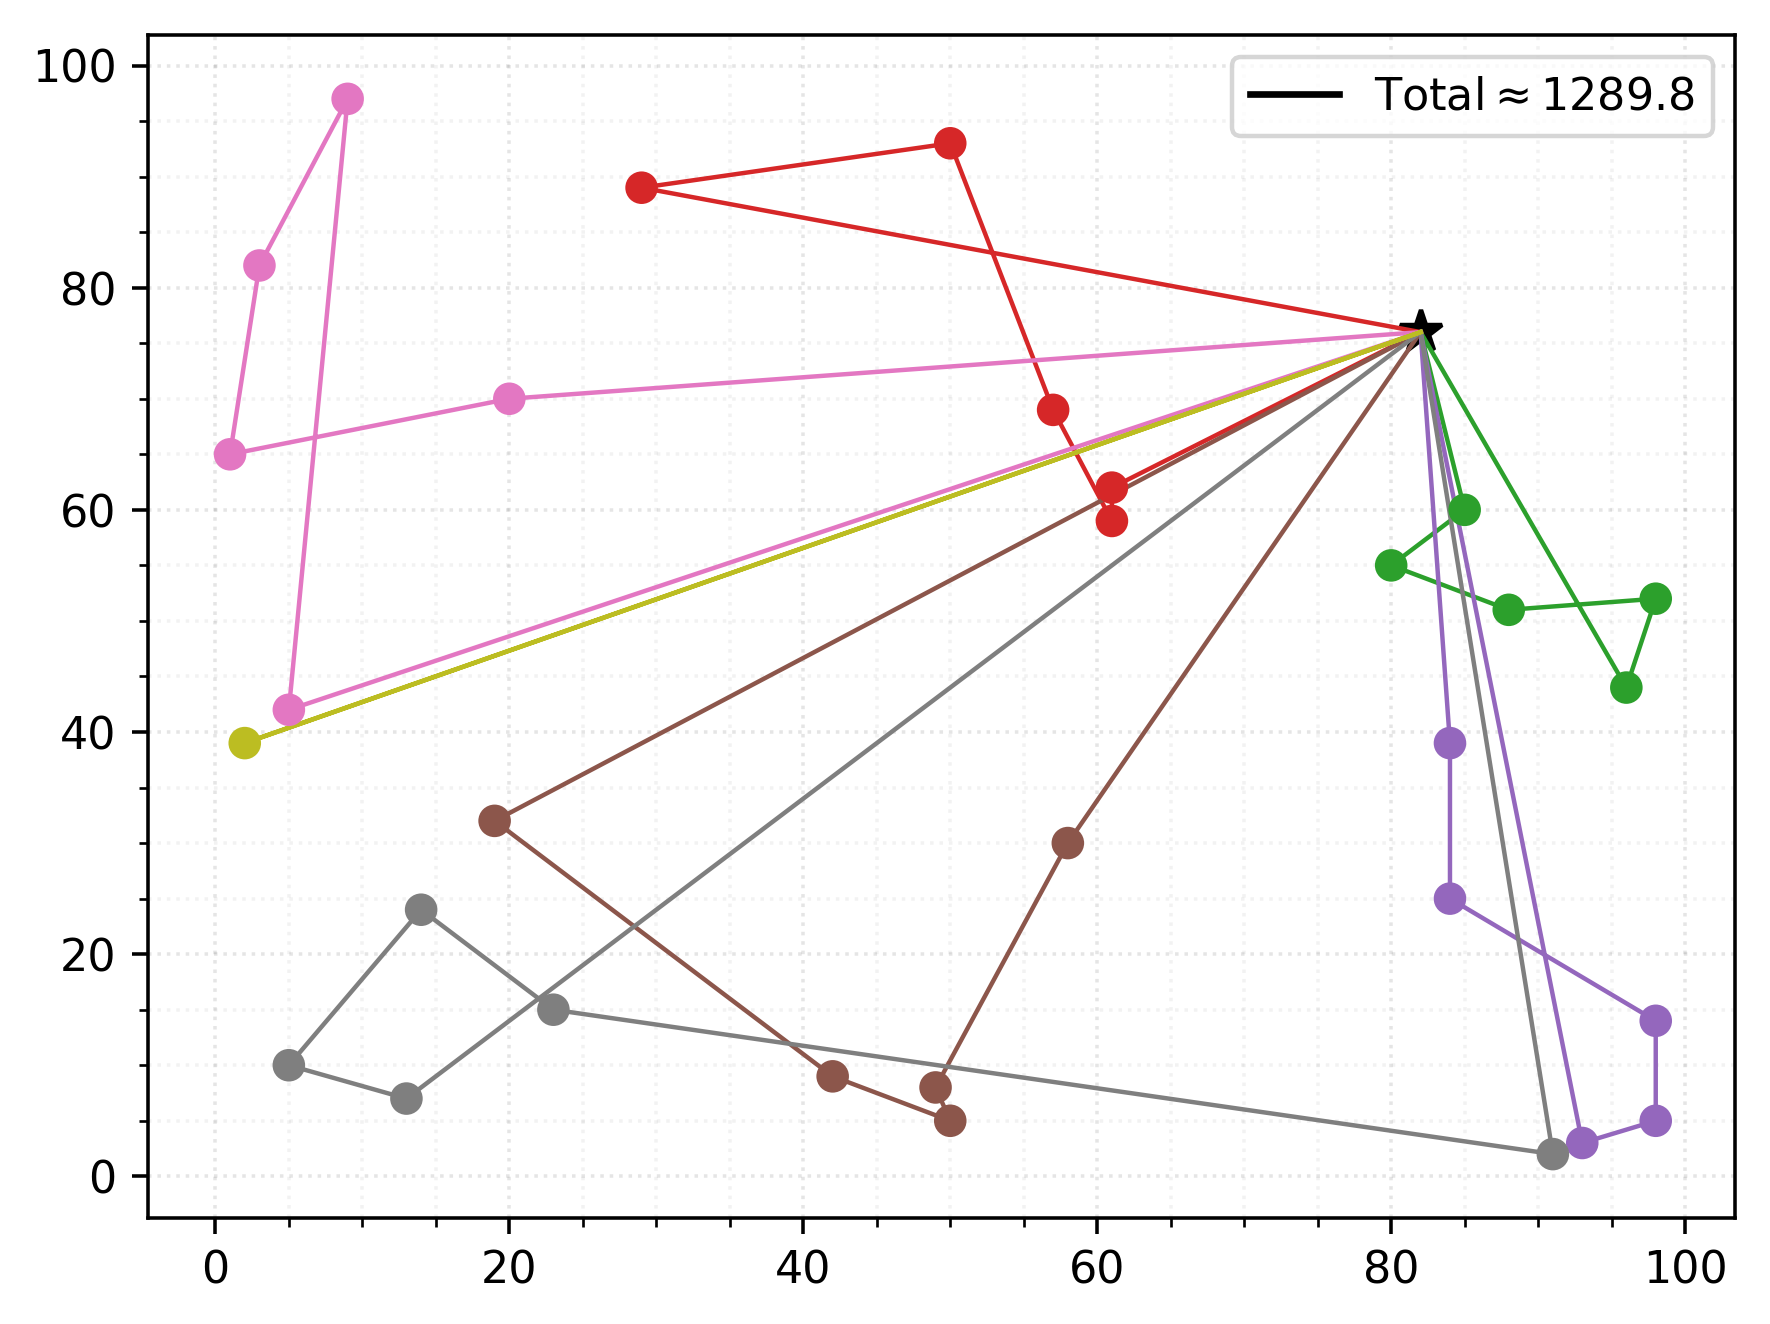
\includegraphics[width=1\textwidth]{greedy/gr-custom-n32-equal-demands-K4}
    \footnotesize \textbf{(b)} $K = 4$
	\end{minipage}%
  \hspace{0.03\textwidth}
	\begin{minipage}{0.30\textwidth}
		\centering
		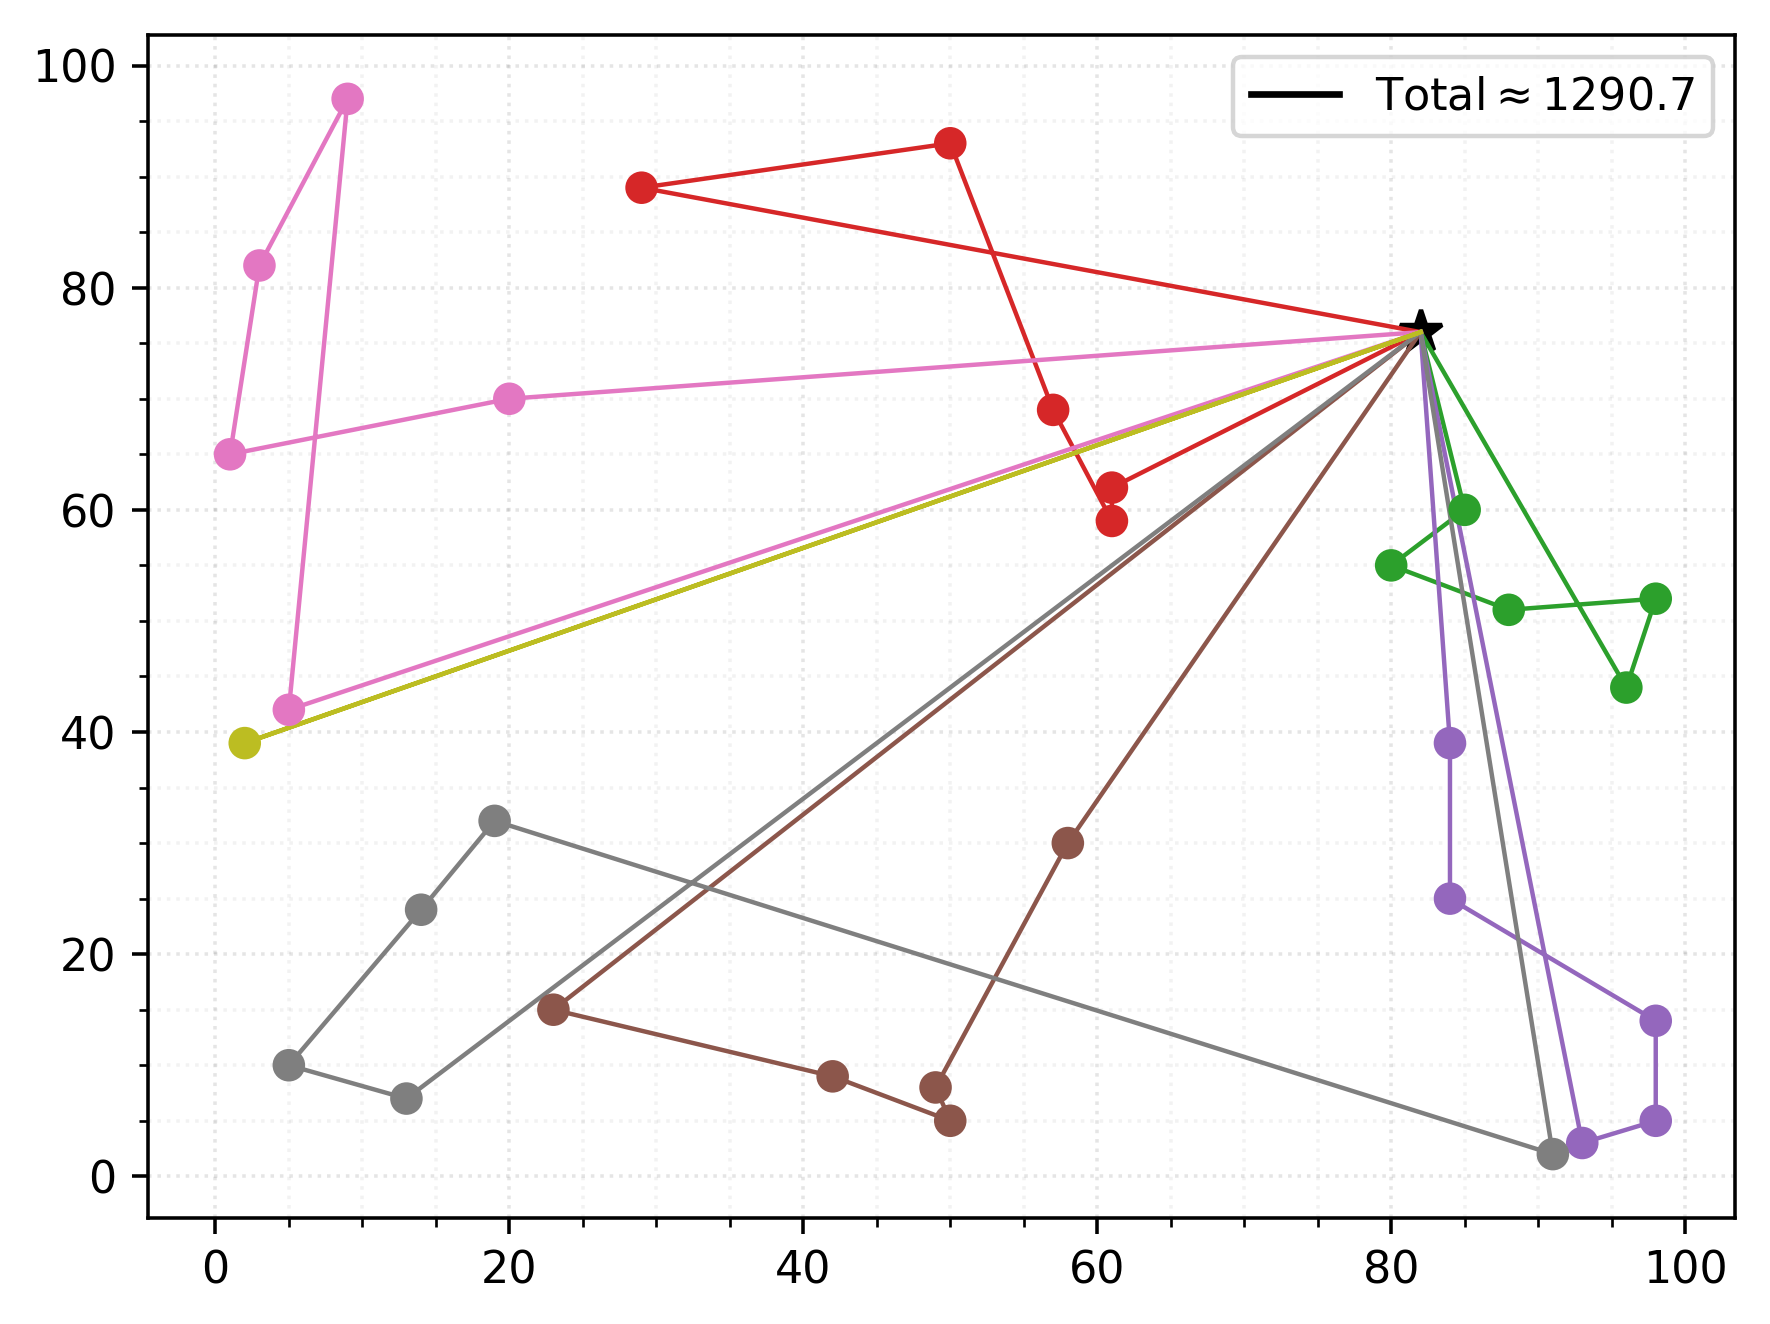
\includegraphics[width=1\textwidth]{greedy/gr-custom-n32-equal-demands-K20}
    \footnotesize \textbf{(c)} $K = 20$
	\end{minipage}%
\end{figure}

Podemos observar que teniendo demandas equivalentes, la heurística golosa sobre demandas es inútil. Sin embargo, podemos observar que los casos \textbf{(b)} y \textbf{(c)} no son tan caóticos como el caso \textbf{(a)}. Esto se debe a que hay otra heurística en juego tomando el protagonismo que la heurística por demanda dejó, y es la que atiende el vértice más cercano al que se está actualmente. Este criterio es el \textbf{paso 4} introducido en la sección \ref{sec:greedy-design}. El comportamiento de este subalgoritmo está atado al valor de $K$ que decidimos fluctuar entre cada solución. En la solución \textbf{(a)} se dispone de un $K=1$, por lo tanto no se explora un vértice más cercano al que se está parado en cada momento. En consecuencia, la planificación de las rutas goza de una distribución imprevisible. Por otro lado, las soluciones \textbf{(b)} y \textbf{(c)} disponen de un valor de $K$ mayor al de \textbf{(a)}, pero una mucho más grande que la otra. Sin embargo, las distancias recorridas son casi equivalentes. Mientras que la diferencia en unidades recorridas entre \textbf{(a)} y \textbf{(b)} es de $206.1$ unidades a favor del último, la diferencia entre \textbf{(b)} y \textbf{(c)} es de $0,9$ a favor de \textbf{(b)}. Esta es una diferencia inquietante por dos razones: la primera, su diminuta magnitud. Y la segunda, que es a favor del caso con un $K=4$ y no $K=20$ como se podría esperar desde un principio. Una explicación plausible es que \textbf{el vértice más cercano no siempre es el más óptimo a largo plazo}.

\subsubsubsection{Demandas incongruentes con el stock de los camiones}
Al mismo tiempo, puede suceder que las elecciones de demandas no hagan un uso óptimo del stock del camión. Imaginemos que tenemos un conjunto ordenado de vértices $V=[v_{1}, v_{2}, v_{3}, v_{4}]$ con demandas $D=[55, 50, 25, 25]$ y un stock máximo de $100$ unidades. Nuestro algoritmo resolvería visitar primero $v_{1}$ con demanda $55$, luego intentaría $v_{2}$ con demanda $50$ pero fallaría y finalmente, con $100 - 55 = 45$ de stock disponible, visitaría $v_{3}$ con una demanda de $25$, dejando un sobrante de stock de $20$ unidades insatisfacibles para el resto de los vértices visitados. En cambio, si el algoritmo no hubiese decidido visitar el nodo más demandante primero y hubiese resuelto visitar $v_{2}$, $v_{3}$ y $v_{4}$ con una demanda total de $100$, no nos sobraría stock y habríamos cubierto tres vértices con un solo camión (en vez de dos como en el caso anterior). El algoritmo no explora posibles soluciones vecinales por lo tanto, en algunos casos, se arriesga a ser ineficiente en la cantidad de camiones y en consecuencia en las distancias recorridas.

\begin{figure}[H]
	\centering
	\begin{minipage}{0.48\textwidth}
		\centering
		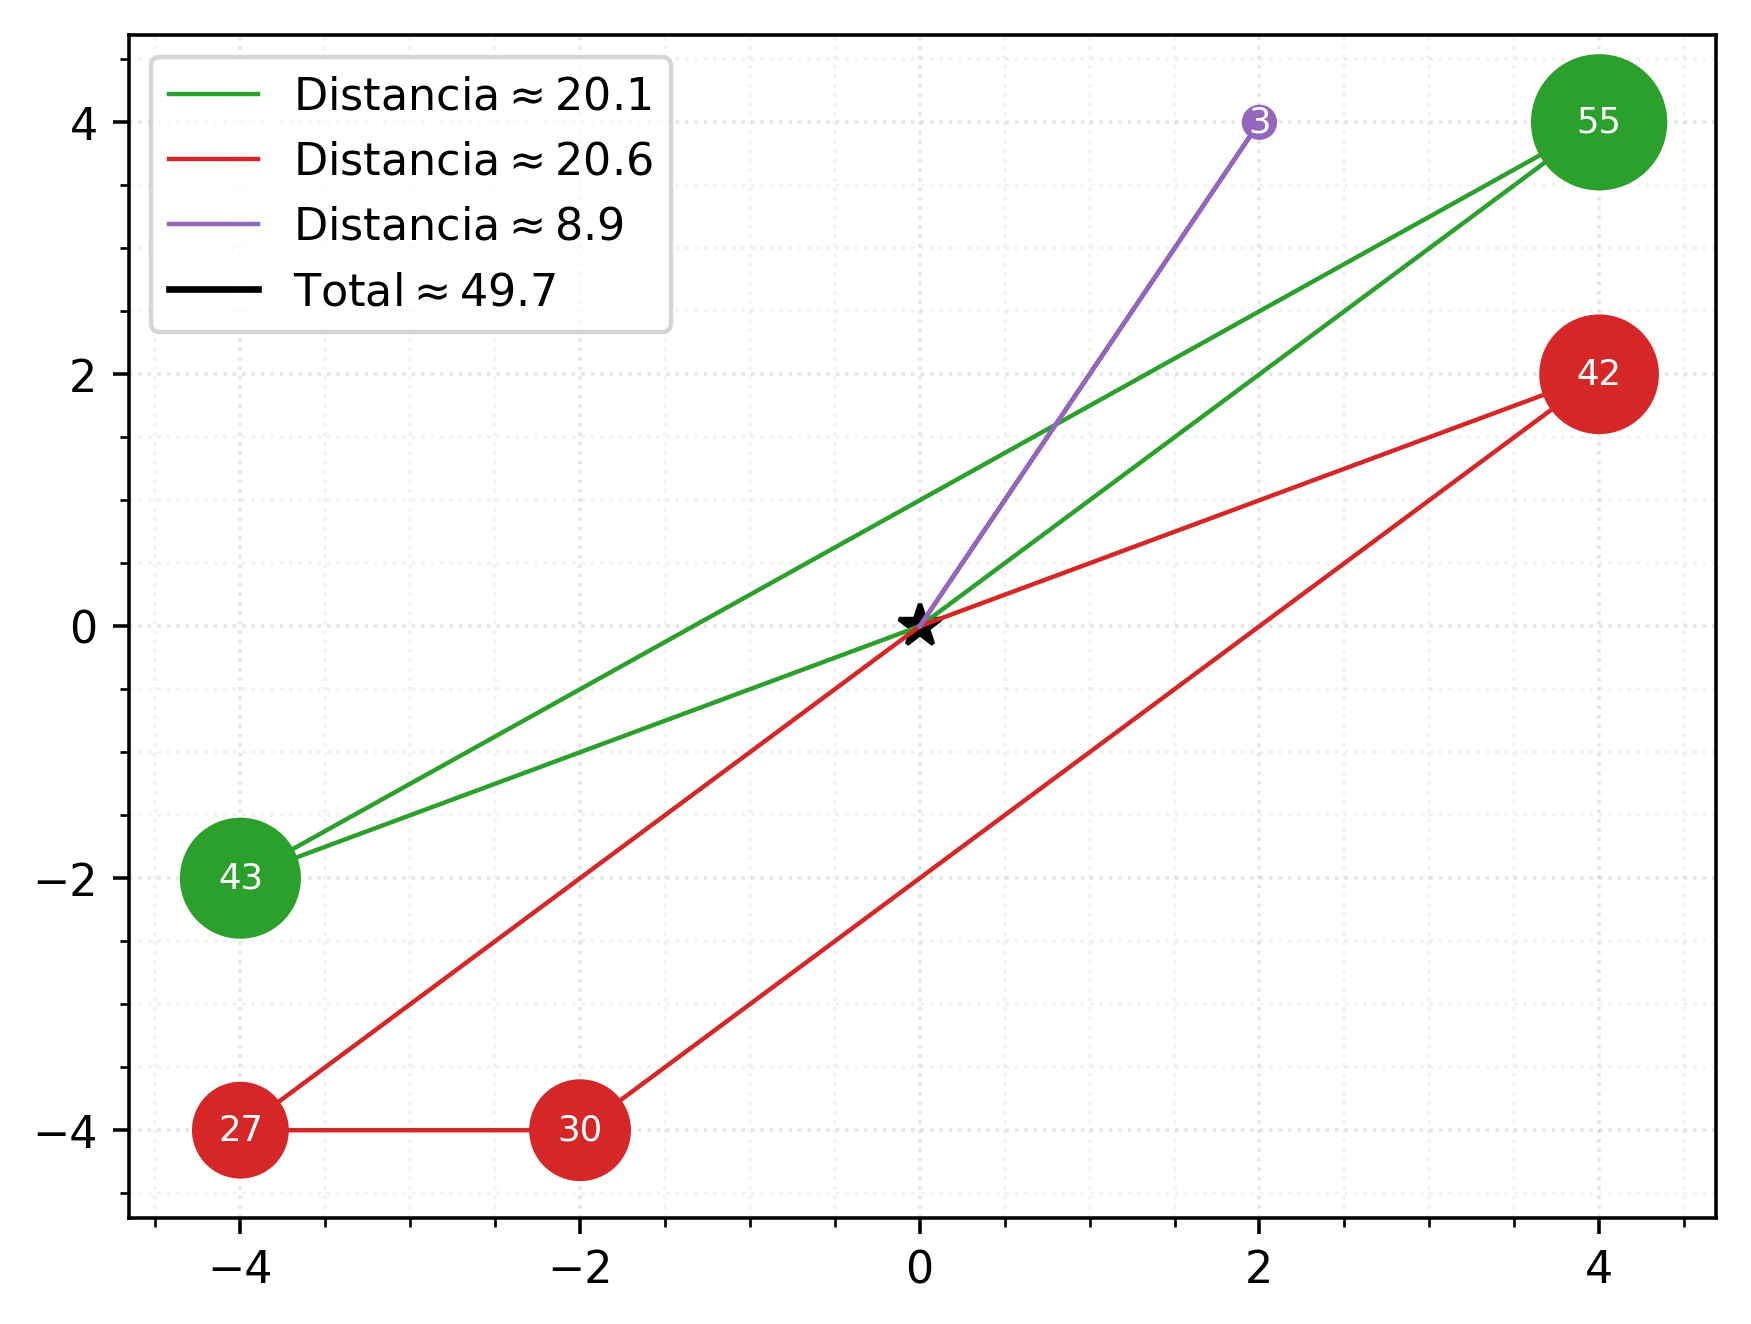
\includegraphics[width=1\textwidth]{greedy/gr-custom-n7-greedy-incongruent-K4}
		\caption{\footnotesize Solución no óptima mediante el algoritmo \textbf{goloso constructivo}. Capacidad 100.}
		\label{fig:gr-custom-n7-greedy-incongruent-K4}
	\end{minipage}%
	\hspace{0.03\textwidth}
	\begin{minipage}{0.48\textwidth}
		\centering
		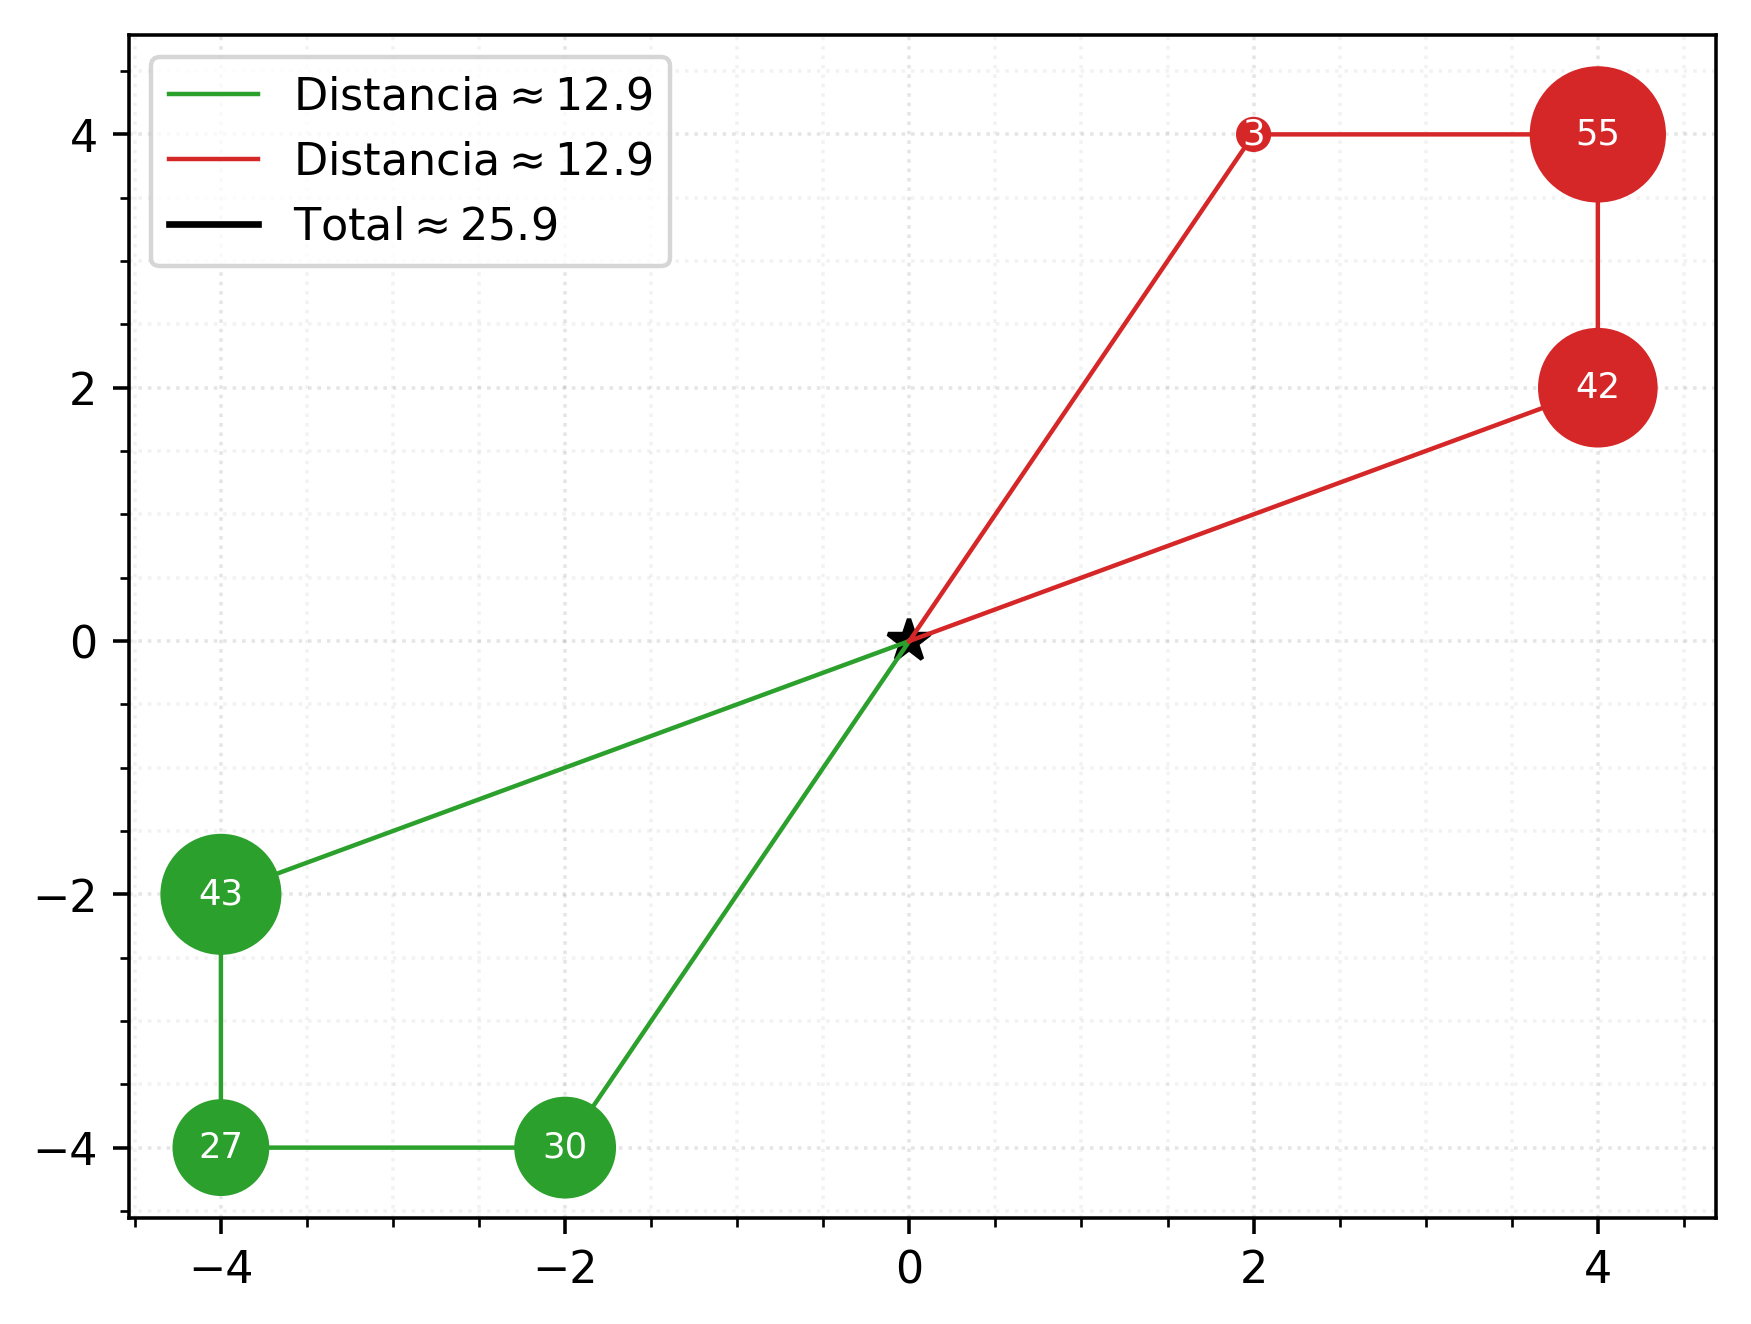
\includegraphics[width=1\textwidth]{greedy/sa-custom-n7-greedy-incongruent}
		\caption{\footnotesize Solución óptima mediante el algoritmo \textbf{Savings}. Capacidad 100.}
		\label{fig:sa-custom-n7-greedy-incongruent}
	\end{minipage}%
\end{figure}

Podemos observar que la solución obtenida con el algoritmo goloso recorre una distancia total de $49.7$ unidades, requiere \textbf{tres camiones} y además de todo, el camión del camino verde finaliza con $2$ unidades de stock sobrante, el camión rojo con $1$ unidad de stock sobrante y el púrpura con $97$ unidades de stock sobrante, dando una suma de $2+1+97=100$ unidades sin proveer. Esto es un gran desperdicio de stock y representa una \textbf{pérdida de oportunidad importantísima}. Por otro lado, el algoritmo de Savings encuentra la solución óptima al problema, utilizando sólo dos camiones, recorriendo la distancia mínima posible y proveyendo la totalidad del stock de todos los camiones. Solución perfecta.

\subsubsubsection{Demanda máxima demasiado grande (limitación de diseño)}
Por una decisión de diseño, se decidió utilizar un \textit{bucket sort} para ordenar las demandas de los vértices en $\mathcal{O}(n)$. Si bien podríamos haber utilizado otro algoritmo en el orden de complejidad $\mathcal{O}(n*log(n))$, \textit{bucket sort} nos proveyó un entorno más cómodo y elegante y debido a que el universo de instancias con las cuales experimentaríamos disponía de un valor de demanda máxima acotada, creímos conveniente optar por esta opción. Sin embargo, podrían existir instancias donde $D$ sea extremadamente grande. Estas afectarían gravemente el consumo de memoria de la computadora y podrían inhabilitar el funcionamiento del algoritmo. En estos data-sets no es el caso.

\subsubsubsection{Distribución adecuada de los pesos}
A pesar de las debilidades del algoritmo, también existen casos favorables para él. Por ejemplo, si los nodos más pesados están naturalmente \textit{clusterizados}, es decir, cercanos entre sí. Veamos un ejemplo:

\begin{figure}[H]
	\centering
	\begin{minipage}{0.48\textwidth}
		\centering
		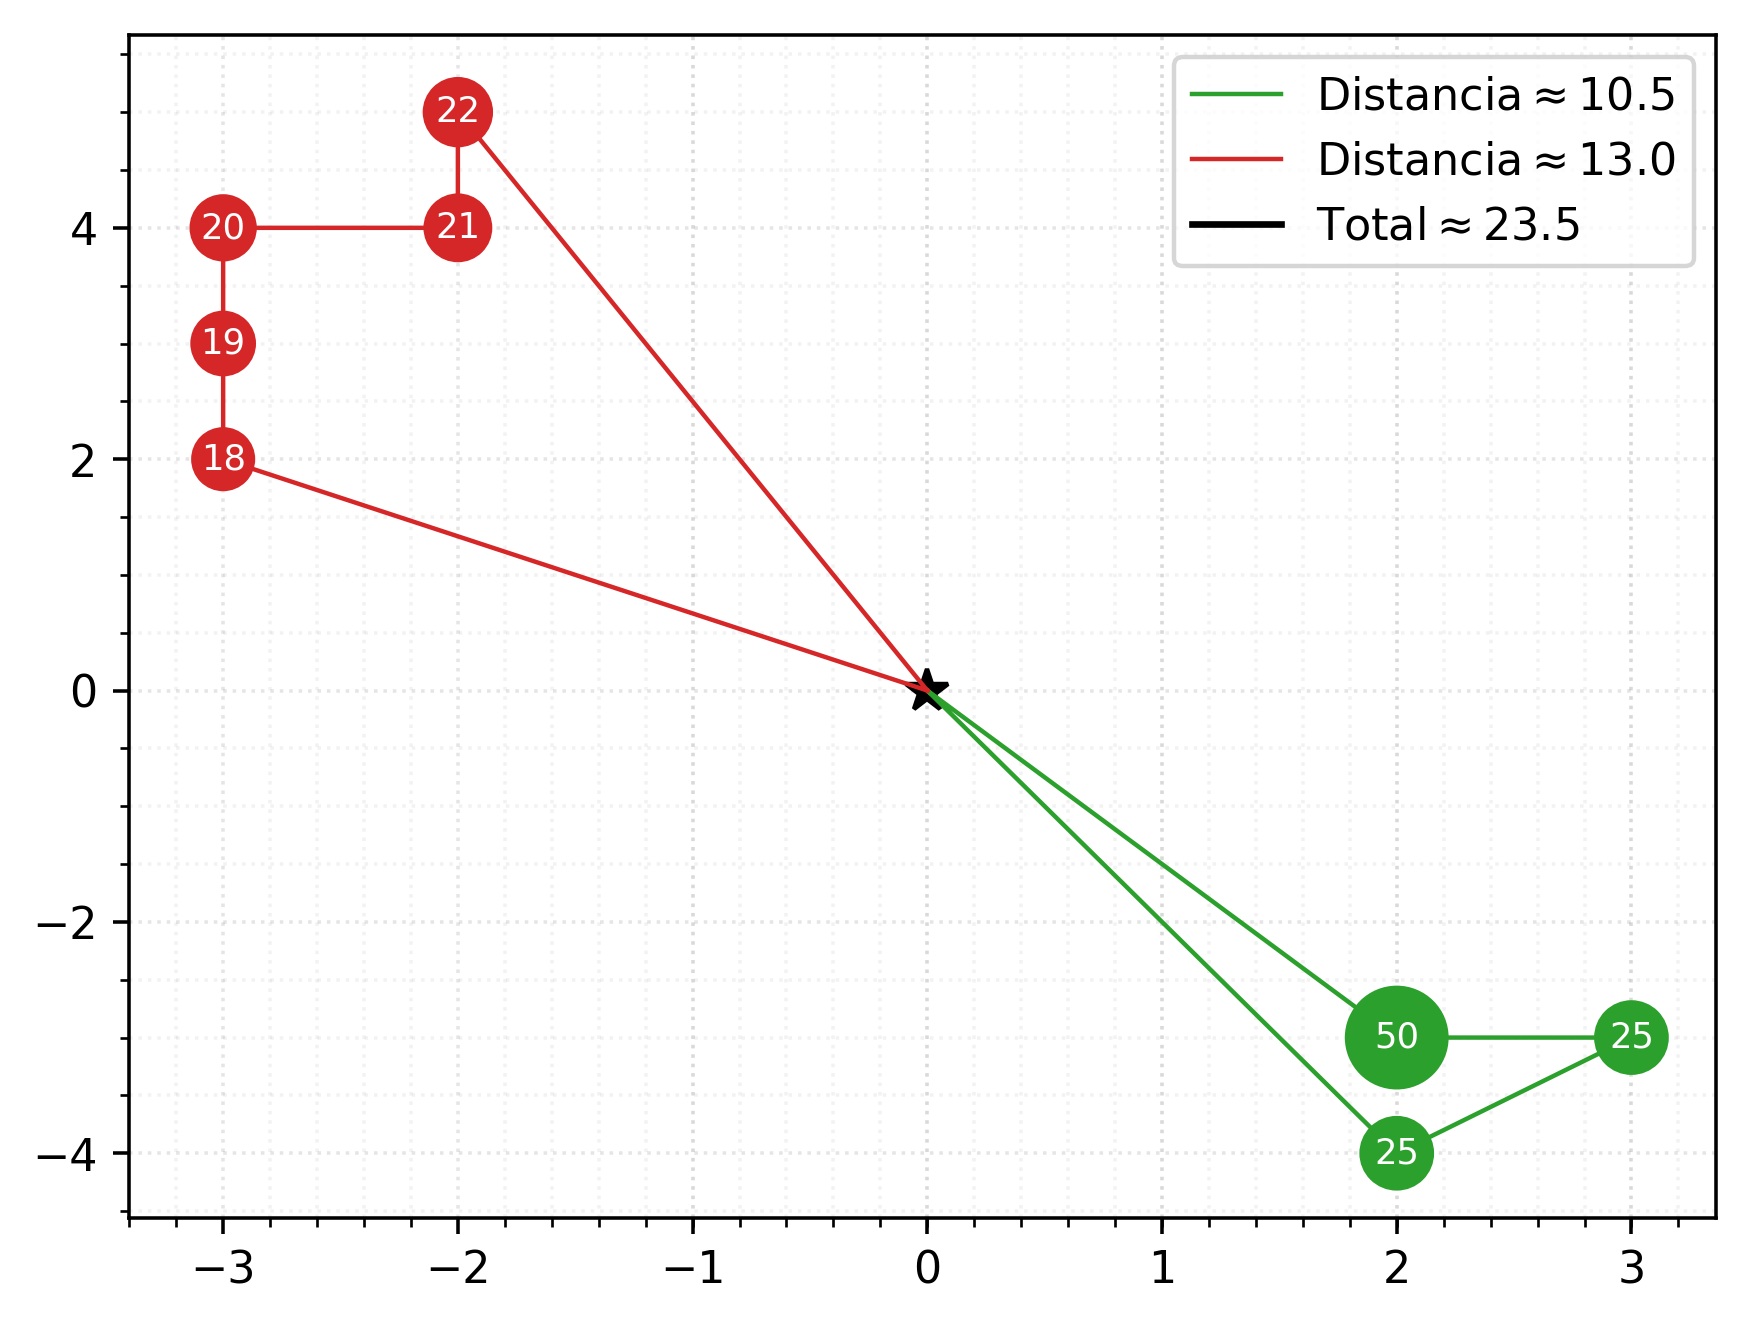
\includegraphics[width=1\textwidth]{greedy/gr-custom-n9-greedy-convenient-K4}
		\caption{\footnotesize Solución golosa constructiva quasi-óptima.}
		\label{fig:gr-custom-n9-greedy-convenient-K4}
	\end{minipage}%
	\hspace{0.03\textwidth}
	\begin{minipage}{0.48\textwidth}
		\centering
		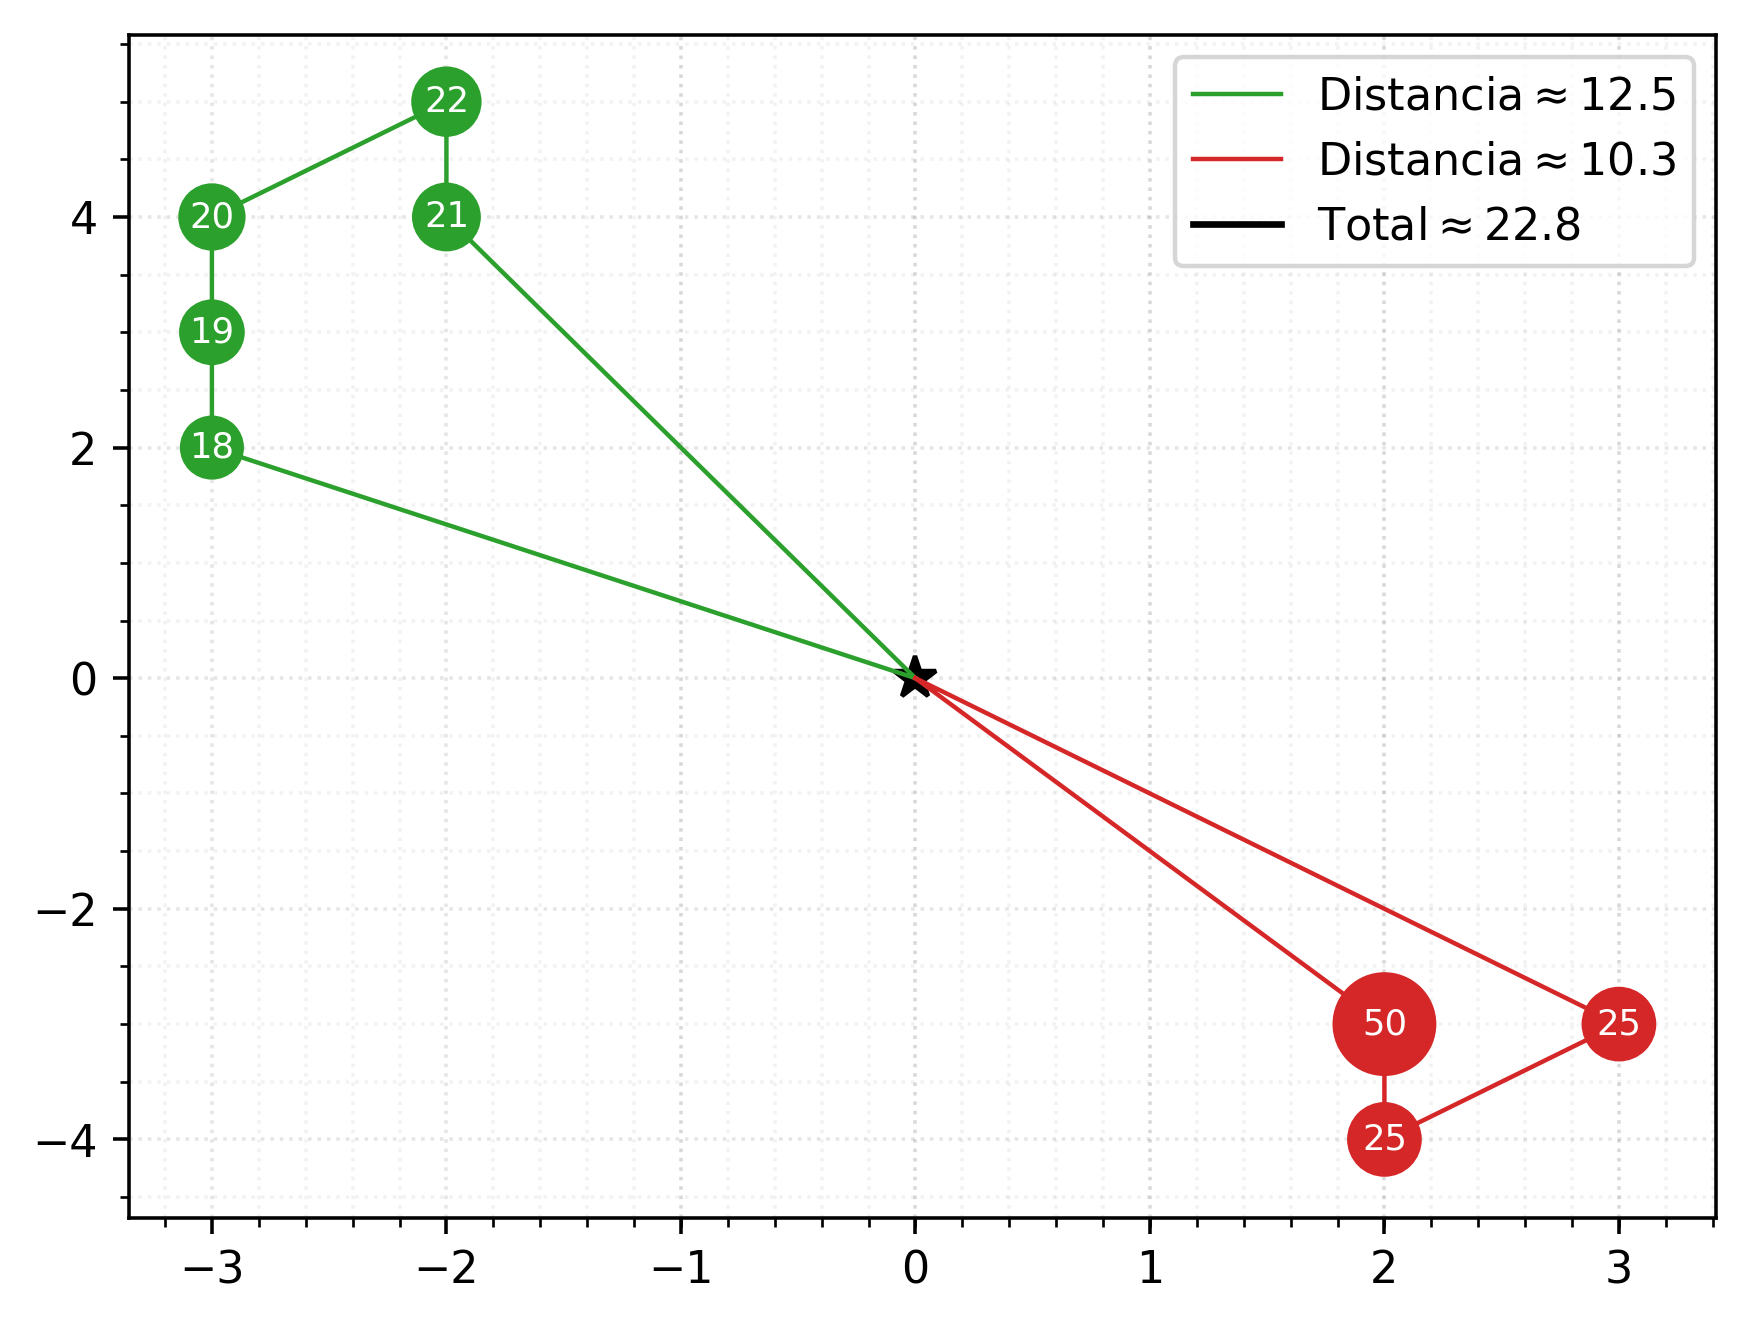
\includegraphics[width=1\textwidth]{greedy/sa-custom-n9-greedy-convenient}
		\caption{\footnotesize Solución óptima con \textbf{savings}.}
		\label{fig:sa-custom-n9-greedy-convenient}
	\end{minipage}%
\end{figure}

Si bien el algoritmo goloso no encuentra la solución más óptima, devuelve un resultado bastante aproximado. No sería dificil fabricar una instancia \textit{ad-hoc} que favorezca a la perfección al algoritmo en cuestión. De este ejemplo podemos concluir que, si bien la heurística constructiva golosa puede ser muy grosera, podrían existir alternativas donde – modificándola adecuadamente – se pueda utilizar para detectar grandes clusterizaciones de demandas (que podrían representar, por ejemplo, una ciudad con muchos clientes muy demandantes) para tomar una decisión inteligente al respecto, como con cuántos camiones intentar proveer ese foco de vértices, etcétera. Esta propuesta excede el alcance de este documento y es mencionada como una posible alternativa \textbf{factible} en donde esta heurística podría convivir a la par de otras más efectivas como Savings y Annealing.
